\chapter{Introduction}

Scientists, engineers, and researchers use wireless sensor networks (WSN) for a wide array of applications. Many of these applications rely on knowledge on the precise position of each node. While some may only require relative coordinates within the network, most biological, geophysical, and other scientific applications require coordinates on a global coordinate system. Perhaps the obvious solution is for each node in the network to be equipped with GPS or other location positioning service.  However, constraints on cost, power consumption, as well as visibility of satellites forbids this.  

Many protocols have been propopsed [TODO refs] to calculate relative positions amongst the nodes of a network.  They vary in the required network functionality in terms of radio ranging or range-free.  However, in all cases, in order to convert from relative to global coordinates, some of the nodes do require a local source of global coordinates by using GPS or some other source.  This can be achieved by operators recording the global coordinates during network deployment or by the device having GPS embedded in a subset of the nodes.  We call these enhanced nodes anchors.  Here, we explore the effect of anchor node placement within the network on the overall localization errors, on a network-wide basis. This provides network planners with a set of general rules to minimize the number of anchor nodes required while avoiding poor node localization, allowing scientists to assume a maximum position error during their own research.


\section{Motivation} 

%\begin{figure} % % Requires \usepackage{graphicx} % \centering %
%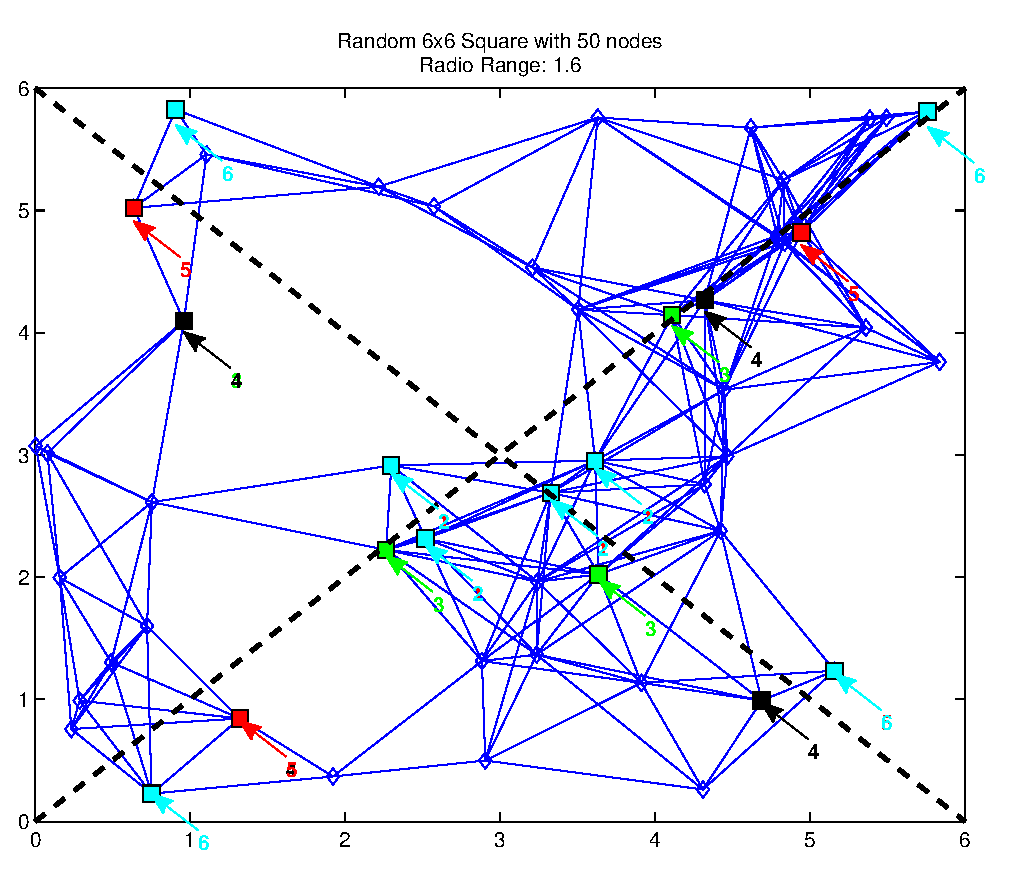
\includegraphics[width=4in]{../cca/results/45DegreeAxis_Random/networkRandom6x6Squarewith50nodes1-6Radius.eps}\\
% \caption{The random network used, showing the 6 position sets of anchors.} %
%\label{fig:45DegreeAxisRandomNetwork} %\end{figure}

%\begin{equation}\label{eqn:newton_law} %    F = Ma %\end{equation}
%Paragraph referencing an equation \ref{eqn:newton_law}.
